\section{Segmentation}
The first step towards graph recognition is segmentation. This step identifies the segmentation points in the input graph. These points are fed into the recognition task to identify a component. Our implementation is based on the idea presented by \citeauthor{daly2015hand} \cite{daly2015hand} and assumes that the entire component is drawn in one stroke. However, drawing multiple components in the same stroke is acceptable for our implementation.\\

The segmentation points identify the transition from one component to the next. These are referred to as true segmentation points.  However, there are certain challenges in the segmentation task. These challenges arise from the fact that there might be additional points in a component with similar geometric properties as true segmentation points. This is shown in Figure \ref{fig:seg_false_neg}. The challenges can be divided into two buckets: false positives and false negatives. The points that are incorrectly identified as segmentation points contribute to false positives. These cases are less severe as they can be handled in the classification step. The points that are true segmentation points but are missed by the segmentation algorithm are false negatives. These cases are more severe as we cannot recover from these errors. The goal of the segmentation algorithm would be to minimize false positives while ensuring that there are no false negatives.\\

\begin{figure}
	\centering
	\begin{subfigure}{0.3\textwidth}
		\centering
		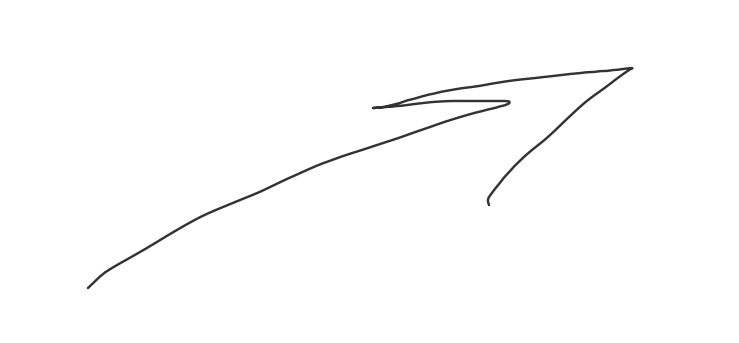
\includegraphics[scale=0.2]{./img/seg_orig.jpg}
	\end{subfigure}
	\begin{subfigure}{0.3\textwidth}
		\centering
		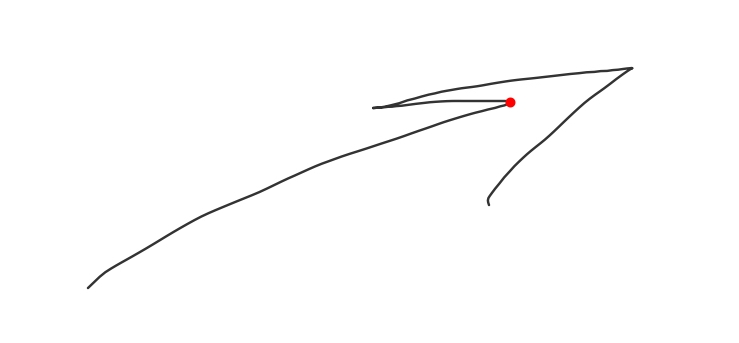
\includegraphics[scale=0.2]{./img/seg_true_seg.jpg}
	\end{subfigure}
	\begin{subfigure}{0.3\textwidth}j
		\centering
		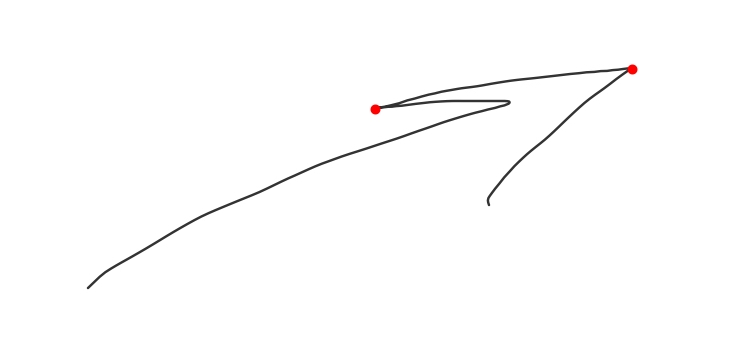
\includegraphics[scale=0.2]{./img/seg_false_seg.jpg}
	\end{subfigure}
	\caption{\textit{left} a line and arrow head drawn in one stroke, \textit{middle} true segmentation point, \textit{right} additional points with similar properties as true segmentation points}
	\label{fig:seg_false_neg}
\end{figure}

\subsection{Algorithm}
We explored two segmentation algorithms for the online recognition problem - curvature-based and speed-based.

\subsubsection{Curvature-Based Segmentation}
The curvature-based segmentation algorithm is based on the observation that there are abrupt changes in curvature at segmentation points. This is based on the properties of transition that can occur in the three types of graph components. This is shown in figure \ref{fig:seg_curvature}.\\

Before the curvature calculation, some pre-processing of input data is required. We use iPyCanvas \cite{ipycanvas} to capture the coordinates of the drawn components. The number of coordinates captured depends on the drawing speed. If the drawing speed is higher in certain regions, the number of points captured will be higher in those region. This count is normalized by considering the distance between two points. If the Euclidean distance between two consecutive points, $P_i$ and $P_{i+1}$, is less than a threshold, $d_t$, we drop $P_{i+1}$. Here, $d_t$ is a hyperparameter that needs to be trained based on the input data.\\

The \textit{curvature} of a point $P_i$ is computed by calculating the angle between the vectors formed by joining $P_{i-s}$ and $P_i$ and $P_i$ and $P_{i+s}$. $s$ is the second hyperparameter.

\begin{equation}
	C_s(P_i) = \arccos \left(  \frac{\overrightarrow{P_{i-s} P_i} \cdot \overrightarrow{P_i P_{i+s}}}{ \Vert \overrightarrow{P_{i-s} P_i}  \Vert \; \Vert \overrightarrow{P_i P_{i+s}} \Vert  } \right) 
\end{equation} 

Once the curvature is computed for all captured points, we compute \textit{abnormality}. This metric is used in identifying the abrupt and significant changes in the curvature. The abnormality of a point $P_i$ is defined by how the curvature at that point differs from the average curvature of the surrounding points.
\begin{equation}
	A_{s,w}(P_i) = C_s(P_i) - \frac{\sum_{j=a}^{i-1} C_s(P_j) + \sum_{j=i+1}^{b} C_s(P_j)}{b - a}
\end{equation}
where $a = max(1, i-w)$ and $b = min(n, i+w)$.\\

$w$ is the third hyperparameter. Next, we need to find ranges of points where $k A_{s, w}(P_i) > 1$ and select the point with maximum abnormality in each range as the segmentation point. The multiplication factor $k$ is the fourth hyperparameter.\\

\begin{figure}
	\centering
	\begin{subfigure}{0.45\textwidth}
		\centering
		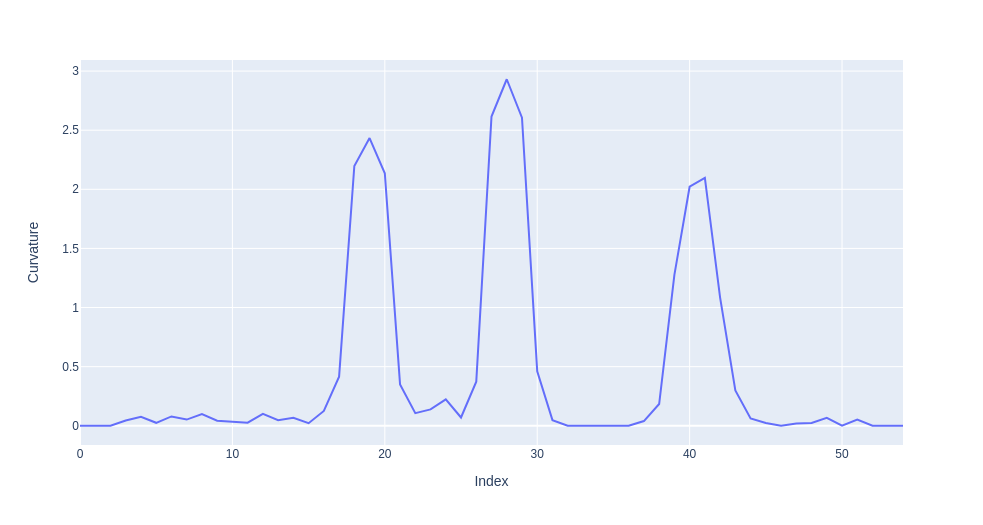
\includegraphics[scale=0.23]{./img/seg_curvature_arrow}
		\caption{Curvature}
	\end{subfigure}
	\hfill
	\begin{subfigure}{0.45\textwidth}
		\centering
		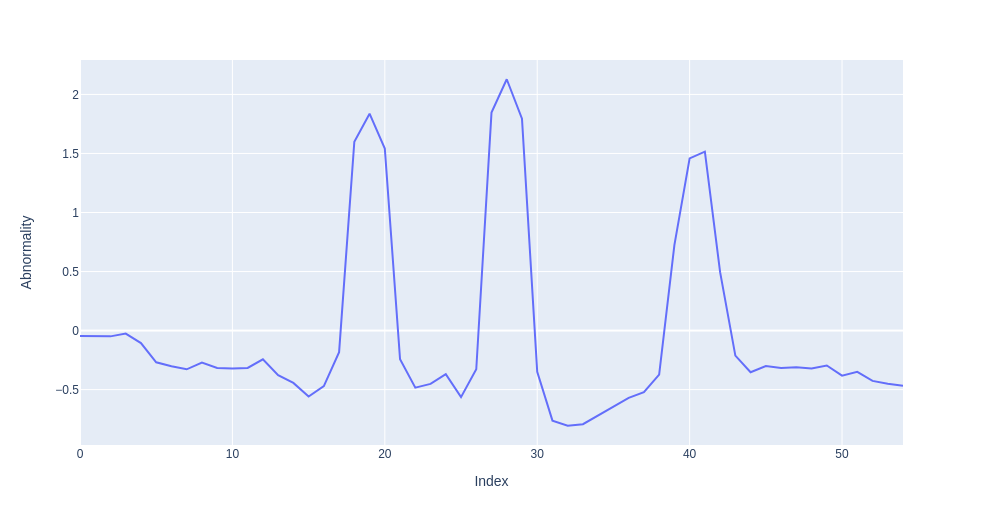
\includegraphics[scale=0.23]{./img/seg_abnormality_arrow}
		\caption{Abnormality}
	\end{subfigure}
	\caption{Curvature and abnormality plots for the components shown in figure \ref{fig:seg_results_arrow}. The peaks represent the segmentation points.}
	\label{fig:seg_curvature}
\end{figure}

\subsubsection{Speed-Based Segmentation}
This algorithm is based on the observation that the drawing speed reduces while drawing corners. We implemented and experimented with a simplified version of the algorithm presented by \citeauthor{wang2021segmentation} \cite{wang2021segmentation}.\\

For every coordinate captured by iPyCanvas, we also recorded a timestamp. The \textit{speed} of stylus for a point $P_i$ is given by
\begin{equation}
	v(P_i) = \begin{cases}
		\frac{\Vert \overrightarrow{P_{i-i} P_i}  \Vert}{t_i - t_{i - 1}} & 0 < i < n - 1\\
		0 & i = 0; i = n-1
	\end{cases}
\end{equation}

Once the speed is computed for all captured points, we find ranges of points where $v(P_i) < V_t$ and select the point with minimum speed in each range as the segmentation point. $V_t$ is a hyperparameter here.\\

After computing the potential segmentation points, we perform a post-processing step to drop the points that are close to each other. This step is similar to the pre-processing step discussed in the curvature-based segmentation algorithm and has a hyperparameter $d_t$.\\

As we would see in subsection \ref{sec:seg_experiments} that this method is not super accurate and produces quite a few false positives. But it is very fast compared to the curvature-based segmentation. In general, the component classification step can take care of false positives. So, if a usecase requires faster computation, this method can be used with a good component classifier to reduce the overall computation time.

\begin{figure}
	\centering
	\begin{subfigure}{0.45\textwidth}
		\centering
		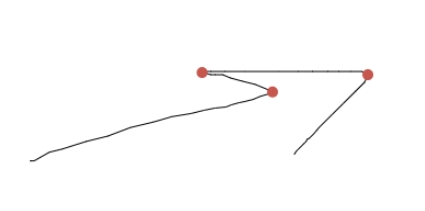
\includegraphics[scale=0.5]{./img/seg_results_arrow.jpg}
		\caption{}
		\label{fig:seg_results_arrow}
	\end{subfigure}
	\begin{subfigure}{0.45\textwidth}
		\centering
		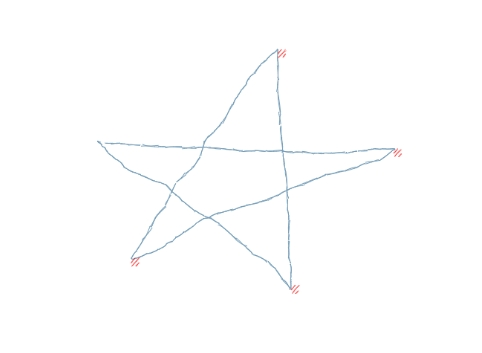
\includegraphics[scale=0.6]{./img/seg_results_pentagram.jpg}
		\caption{}
		\label{fig:seg_results_pentagram}
	\end{subfigure}
	\caption{Curvature-based segmentation algorithm. The segmentation points are highlighted in red.}
	\label{fig:seg_results}
\end{figure}

\begin{figure}
	\centering
	\begin{subfigure}{0.45\textwidth}
		\centering
		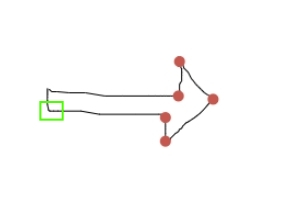
\includegraphics[scale=0.5]{./img/seg_results_arrow_missing.jpg}
		\caption{}
	\end{subfigure}
	\hfill
	\begin{subfigure}{0.45\textwidth}
		\centering
		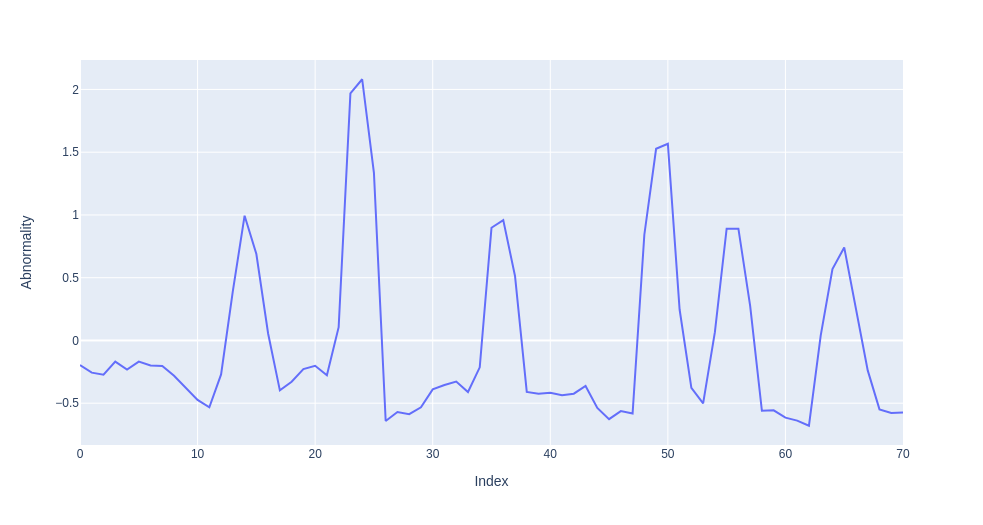
\includegraphics[scale=0.25]{./img/seg_abnormality_arrow_missing}
		\caption{}
	\end{subfigure}
	\caption{False-negative with the curvature-based segmentation: (a) The green box shows a false-negative. (b) The abnormality graph for the stoke.}
	\label{fig:seg_false_negative}
\end{figure}

\begin{figure}
	\centering
	\begin{subfigure}{0.45\textwidth}
		\centering
		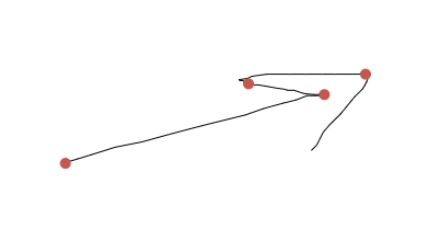
\includegraphics[scale=0.4]{./img/seg_results_arrow_speed.jpg}
		\caption{}
		\label{fig:seg_results_arrow_speed}
	\end{subfigure}
	\begin{subfigure}{0.45\textwidth}
		\centering
		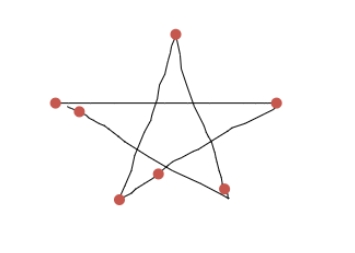
\includegraphics[scale=0.5]{./img/seg_results_pentagram_speed.jpg}
		\caption{}
		\label{fig:seg_results_pentagram_speed}
	\end{subfigure}
	\caption{Speed-based segmentation algorithm. The segmentation points are highlighted in red.}
	\label{fig:seg_results_speed}
\end{figure}

\begin{figure}
	\begin{subfigure}{0.45\textwidth}
		\centering
		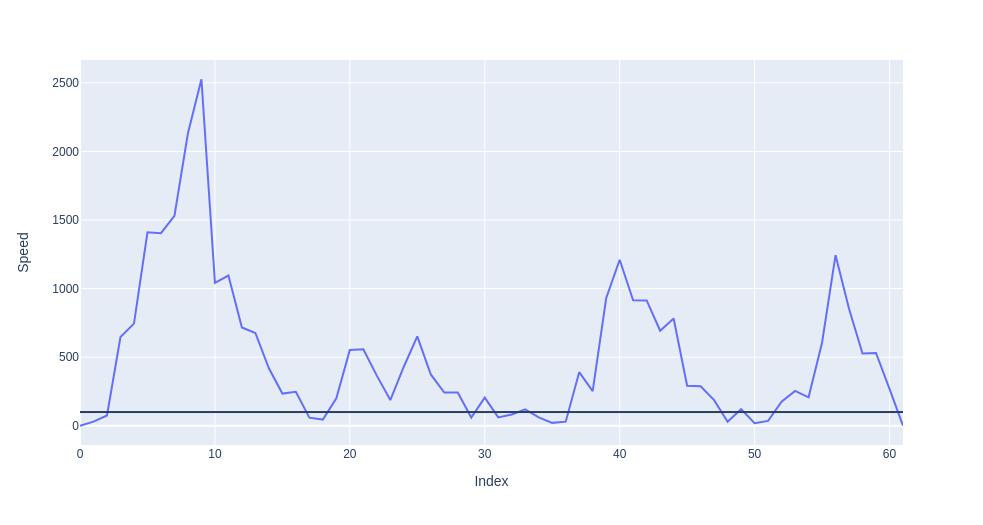
\includegraphics[scale=0.25]{./img/seg_speed_arrow}
		\caption{}
	\end{subfigure}
	\hfill
	\begin{subfigure}{0.45\textwidth}
		\centering
		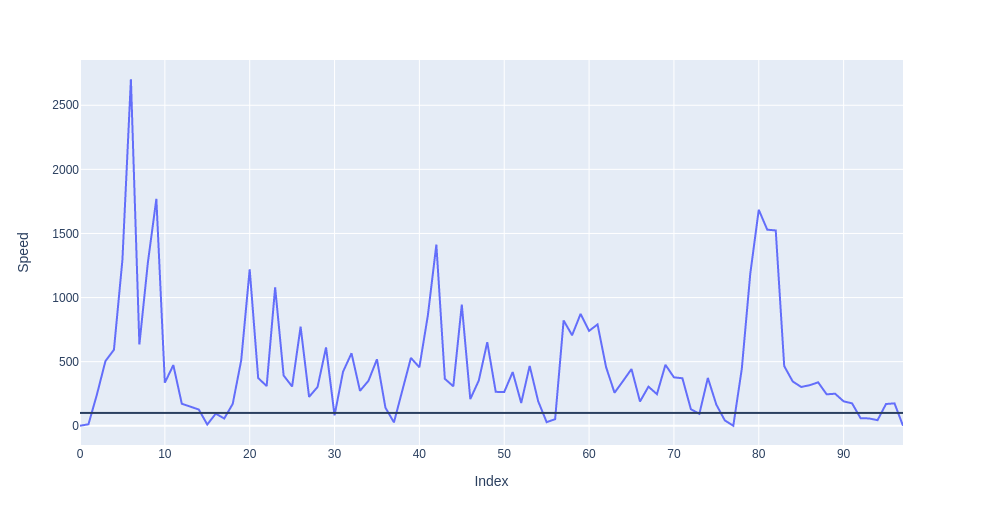
\includegraphics[scale=0.25]{./img/seg_speed_pentagram}
		\caption{}
	\end{subfigure}
	\caption{Speed plots for (a) arrow \ref{fig:seg_results_arrow_speed} (b) pentagram \ref{fig:seg_results_pentagram_speed}. The black line shows the threshold. Points below this line are potential segmentation points.}
	\label{fig:seg_speed_plots}
\end{figure}

\subsection{Experiments}
\label{sec:seg_experiments}
To test the segmentation algorithm, we drew some components and shapes manually on iPyCanvas and validated the results.\\

Figure \ref{fig:seg_results} shows the detected segmentation points for the curvature-based segmentation algorithm. Figure \ref{fig:seg_curvature} shows the curvature and abnormality plots for the stoke in figure \ref{fig:seg_results_arrow}. We also observed cases where a segmentation point was missed by this algorithm. This is shown in figure \ref{fig:seg_false_negative}. The abnormality plot shows all peaks correctly, but the last peak is below the threshold. Hence, the hyperparameter tuning is a critical step for this algorithm. Based on our experiments, the following values of hyperparameters worked best - $d_t = 2$, $s = 3$, $w = 12$, and $k = 1.2$.\\

Figure \ref{fig:seg_results_speed} shows the detected segmentation points for the speed-based segmentation algorithm. Figure \ref{fig:seg_speed_plots} show the corresponding speed plots. It is apparent that this algorithms produces a lot of false-positives. Based on our experiments, the following values of hyperparameters worked best - $V_t = 100$ and $d_t = 10$\\

The execution time for both algorithms is shown in table \ref{table:exec_time}.

\begin{table}[h]
	\centering
	\begin{tabular}{|c|c|c|}
		\hline
		Stroke & Curvature-Based & Speed-Based\\
		\hline
		Arrow & 3.38 ms ± 28.9 µs & 555 µs ± 15 µs\\
		\hline
		Pentagram & 8.77 ms ± 779 µs & 973 µs ± 24.4 µs\\
		\hline
	\end{tabular}
	\caption{Execution time}
	\label{table:exec_time}
\end{table}

Based on the number of false-positives and false-negatives, we used the curvature-based segmentation algorithm in our graph recognition pipeline.